\documentclass[paper-main.tex]{subfiles}


\begin{document}


 
% Tracking tones with the Viterbi algorithm
% explaination and successful application
% lean on the continuous gravitational waves angle
Continuous wave signals may wander slowly in frequency over time. 
%As also mentioned in Section~\ref{sec:introduction}, continuous wave searches often look for signals that wander slowly in frequency~\cite{ScoX1O2Viterbi:2019}. 
The audio analogue of this is a tone that wanders in frequency; a note that changes pitch. 
Unlike the single tone described in Section~\ref{sec:single_tone}, finding the signal isn’t as simple as searching for a peak in the spectrum for the full timeseries data.%observing run.


\han{should we add some more astro details here about LMXBs and why we think they wander in frequency?}

The data from a gravitaitonal wave observation run can be many months to a year. 
One method to search for a slowly wandering continuous wave signal is to split the data into several shorter intervals. 
Each chunk is analysed seperately. 
In our project we take a Fourier transform of each interval and then create a grid (or spectrogram) where each cell is the Fourier amplitude of a particular frequency at a particular time. 
(In continuous wave searches, a detection statistic is used to calculate the probability of a signal being present in a particular frequency bin.)
The task is then to find the best path through the spectrogram grid as if it where a weighted graph, where here the weights are the Fourier amplitudes. 
The Viterbi algorithm~\cite{Viterbi:1967} is an efficient method find the best path through the grid. 
It is used in contiuous wave searches for a range of astrophysical targets~\cite{ScoX1O2Viterbi:2019,ScoX1ViterbiO1:2017,MillhouseStrangMelatos:2020,PostMergerRemnantSearch:2019,SunEtAlSNR:2018,viterbi_application}. 




\subsection{The Viterbi algorithm}

%Here we overview the Viterbi algorithm and describe its usage in this work. 

Abstractly speaking, the algorithm is given a weighted graph (e.g.\ the spectrogram grid), a sensible sequence of subgraphs (e.g.\ the columns of the spectrum at each time), and restrictions on connectivity (e.g.\ the allowed amount frequency wander). 
n, at each iteration, it will find the best path to each node in the next subgraph, all the way from the first subgraph. 
At the end, it selects the overall best path from the first to the last subgraph (here, from the start to end time), this overall best path is called the Viterbi path. 
See Appendix~\ref{app:viterbi} for the full details of the algorithm in this particular implementation.

% moved from above
The method requires a limit for the allowed frequency change over time, usually informed by a physical model. 
Here, the frequency wander limit is set to $0.11\,{\rm Hz}$ which corresponds to one frequency bin per every time bin. 
In some cases, we see this proves poorly adjusted to the signal. 

\subsection{Results}

A wandering frequency signal is played by the speaker and the output recorded via webcam as in Section~\ref{sec:single_tone}.
Note that when creating a wandering frequency signal, the phase change must be integrated up over time, as detailed in Appendix~\ref{app:phase_gotcha}.

\begin{figure*}
	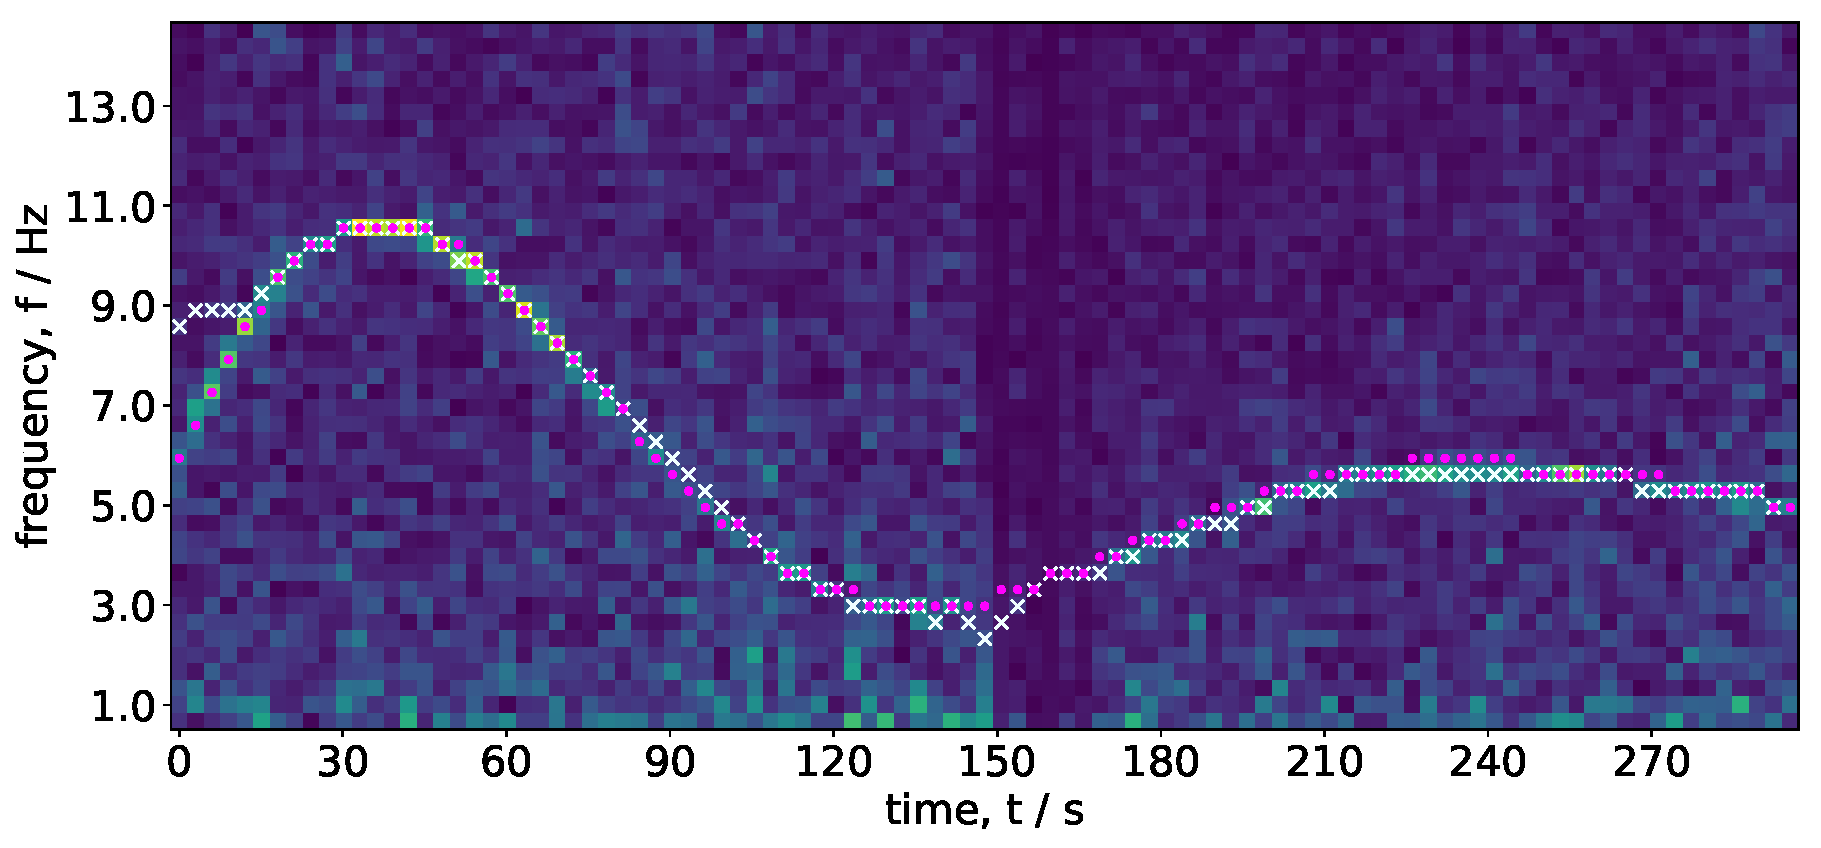
\includegraphics[width=\textwidth]{figures/expt_overlay_2_viterbi_test_webcam.pdf}
	\caption{Results of playing a wandering tone into the interferometer. The spectrogram shows the observed freuqncy amplitudes at each time-frequency step. The overlaid pink dots and white crosses show the injected signal and recovered Viterbi path respetively. At the start (before $\sim 15\,{\rm s}$) the signal changes frequency too quickly for the Viterbi algorithm to recover. At $150\,{\rm s}$ there the data appears anomalous, which may be due to some background noise. }
	\label{fig:viterbi_overlay}
\end{figure*}

Our results are shown in Figure~\ref{fig:viterbi_overlay}, where the heatmap shows the spectrogram of the observed signal. 
The overlaid pick-dot and white-cross markers show the injected signal and recovered Viterbi path respectively. 
To the eye, the Viterbi algorithm easily recovers the injected frequency over time due to the high signal-to-noise ratio (SNR) of this experiment \han{What was the SNR? / can we quantify this?}.
The Viterbi path stays within one frequency bin (approximately $0.3\,{\rm Hz}$) of the injected tone for $94\%$ or the run. \han{Should within one bin be the same as the wander limit above?}
Note that the signal initially moves faster than the frequency wander limit, causing a discrepancy between the injected and recovered signals. 
To fix this, the limit should be doubled, although this would then cause the recovered path to stray more often. 
There also appears to be an anomaly at $150\,{\rm s}$, likely from a disturbance (such as someone walking) around the interferometer.

Empirically, decreasing the signal-to-noise ratio closer to unity (by making the speaker quieter) causes the Viterbi algorithm to stray more from the signal. 
However, since the only correlation through the grid is the signal, we always expect the Viterbi path to lie near to the signal no matter how high the noise is, and this is indeed what we see. \han{Should we show results for this?}


\end{document}
